%****************************************************
%	CHAPTER 2 - LITERATURE REVIEW
%****************************************************
\chapter{Literature Review}
\label{chap:litReview}
%====================================================
\section*{Introduction} \label{sec:litReview.intro}
% Introduce the main differences between Arctic and Antarctic conditions and refer to the problems with existing models & their application to the Antarctic.
% Compare the geographies & ice formation types of the arctic and antarctic to explain the differences
%UPDATE
This chapter aims to introduce and discuss all the relevant literature associated with the subject matter of this project as well as focus on the areas discussed in the problem statement in Section \ref{sec:intro.problemstatement}. This literature review will begin by introducing the climate of the Antarctic continent and the \ac{so} and discussing their importance to the global climate, as well as the ways in which these interact. As discussed in Section \ref{sec:intro.problemstatement}, the differences between the Antarctic and Arctic will be compared and it will be evident from the differences between the two geographies, environment, and interactions with external features, that the two polar regions are vastly different. After discussing the differences between, and different types of ice in, the two regions, the way in which \ac{sar} can be used to characterise sea ice in both regions will be introduced. The focus of this literature review will be on the use of \acs{sar} in the Antarctic region, however, Arctic modelling methods will be examined, and with knowledge of the differences between the two regions, the shortcomings of applying Arctic models to Antarctica will be discussed. Finally, the existing process that is used by the \ac{irea} will be introduced, as well as the history of this method to model sea ice using \acs{sar}.
%====================================================
\section{Antarctic Climate} \label{sec:litReview.antarcticClimate}
% Importance of the Antarctic to world climate and touch on how the climate differs from the Arctic
% In note book
%The Antarctic climate is unique in a global context. In winter, the climate of Antarctica is a particularly limiting factor due to the fact that the sea ice extends far beyond the continent and is inaccessible to ice-breaking ships \cite{Maksym2012}. It is crucial that this limitation is overcome, as the study of the Antarctic climate is important to understand global climate variability and changes \cite{Kennicut2019}.

%This section aims to briefly frame the importance of Antarctica in understanding global climate before focusing on the impact of sea ice and the \acs{miz} on Antarctic climate. As this project focuses on the study of sea ice in the \acs{so}, the following chapter will discuss the theory that is introduced in the following sections with regards to the \acs{miz}, sea ice-ocean interactions, as well as dynamics of the \acs{so} that are important with regard to global climate changes and variation.  

The Antarctic climate holds a unique position within the global context. During the winter, Antarctica's climate poses significant limitations, primarily due to the extensive reach of sea ice beyond the continent, rendering it inaccessible to ice-breaking ships \cite{Maksym2012}. Overcoming this limitation is crucial, as comprehending the Antarctic climate holds significance in understanding global climate variability and changes \cite{Kennicut2019}.

This section aims to provide a concise overview of Antarctica's significance in understanding global climate dynamics. It will subsequently introduce the influence of sea ice and the \ac{miz} on the Antarctic climate. Given the project's focal point on investigating sea ice in the \acs{so}, the subsequent chapter will explore the theories introduced in the upcoming sections. This discussion will encompass the \acs{miz}, interactions between sea ice and the ocean, as well as \acs{so} dynamics that hold significance in the context of global climate changes and variations.

%The contribution of Antarctica to the global climate is due to Antarctic ice sheets, the \acs{so}, and the sea ice that sits on top of it \cite{Kennicut2019}. The Antarctic ice sheets contribute to global sea levels and this contribution has increased in recent years \cite{Kennicut2019}. It is predicted that by the year 2100, the melt of Antarctic sea ice will cause a global sea-level rise of up to 1\,m \cite{Bronselaer2018}. The primary contributor to this ice melt is basal melt\footnote{Basal melting is a result of warmer water being present below an ice sheet and increasing melting from below the ice \cite{Gamache2015}. Lazeroms et al. have observed this in Western Antarctica where warmer seawater has flown into shallower continental shelves beneath ice sheets and sea ice \cite{Lazeroms2018}} which causes the thinning of the ice shelves \cite{Kennicut2019}.

The contribution of Antarctica to the global climate is attributed to the Antarctic ice sheets, the \acs{so}, and the sea ice that blankets it. The Antarctic ice sheets have a significant impact on global sea levels, and this influence has escalated in recent years \cite{Kennicut2019}. Predictions indicate that by the year 2100, the melting of Antarctic sea ice could lead to a global sea-level rise of up to 1\,m \cite{Bronselaer2018}. The primary driver of this ice melt is basal melting\footnote{Basal melting results from the presence of warmer water beneath an ice sheet, intensifying melting from beneath the ice \cite{Gamache2015}. Lazeroms et al. have documented this phenomenon in Western Antarctica, where warmer seawater has intruded into shallower continental shelves beneath ice sheets and sea ice \cite{Lazeroms2018}} leading to the thinning of the ice shelves \cite{Kennicut2019}.

%The large, unbounded \acs{so} has a significant role in the regulation of global climate \cite{Kennicut2019} due to the fact that the \acs{so} stores a large amount of anthropogenic heat\footnote{Anthropogenic heat can be defined as excess heat generated through the direct consumption of energy by human activities. A global database of anthropogenic heat has been constructed by Dong et al. \cite{Dong2017} }, along with greenhouse gasses - mainly carbon dioxide \cite{Kennicut2019}. Furthermore, the \acs{so} forms an integral part of global ocean overturning circulation due to its undersea geography \cite{Thomas2017}. Sea ice in the \acs{so} plays an important role in the overturning circulation as it is a barrier between the strong westerly winds and the ocean surface, as well as managing the density of the \acs{so}. The mechanisms behind this heat storage and circulation are described in Section \ref{sec:theory.soHeat}, whilst the interactions between sea ice and \acs{so} are investigated further in the following sub-sections.

The vast and unbounded \acs{so} plays a significant role in regulating the global climate. This is due to the fact that the \acs{so} acts as a reservoir for a substantial amount of anthropogenic heat\footnote{Anthropogenic heat can be defined as the excess heat generated through the direct consumption of energy by human activities. A comprehensive global database of anthropogenic heat has been constructed by Dong et al. \cite{Dong2017}.}, in addition to greenhouse gases - primarily carbon dioxide \cite{Kennicut2019}. Additionally, the \acs{so} is a crucial component of the global ocean overturning circulation due to its unique underwater geography \cite{Thomas2017Chap8}.

Sea ice within the \acs{so} plays a pivotal role in this overturning circulation as well as modulating heat exchanges \cite{Massom2010}. It acts as a barrier between the strong westerly winds and the ocean surface, while also managing the density of the \acs{so}. The mechanisms underlying this heat storage and circulation are elaborated upon in the theoretical development chapter, whereas the interactions between sea ice and the \acs{so} are explored further in the subsequent sub-sections.

% Last 2 paragraphs to top (adapt) - to do an intro on why we care about Antarctica 
% Sea ice section/compare to Arctic
% At the end of the intro, mention what I want to discuss, and why I am discussing it - why do I care to read on (FRAME NICELY)

\subsection{Antarctic Sea Ice} \label{subsec:litreview.antarctica.seaIce}

The extent of the sea ice in Antarctica varies significantly, between a seasonal maximum of 19 million\,km$^2$ during winter and a minimum of 3-4 million\,km$^2$ - a range of more than 1.5 times larger than the seasonal changes in the Arctic \cite{Thomas2017Chap8}. The seasonal sea ice extent is shown in Figure \ref{fig:litReview.antarcticClimate.seaIceExtent2022}. %The importance of sea ice in Antarctica is discussed in the following sub-section, with comparisons between the Arctic and Antarctic also considered.

\begin{figure}[H]
	\centering
	\begin{subfigure}[t]{.48\linewidth}
		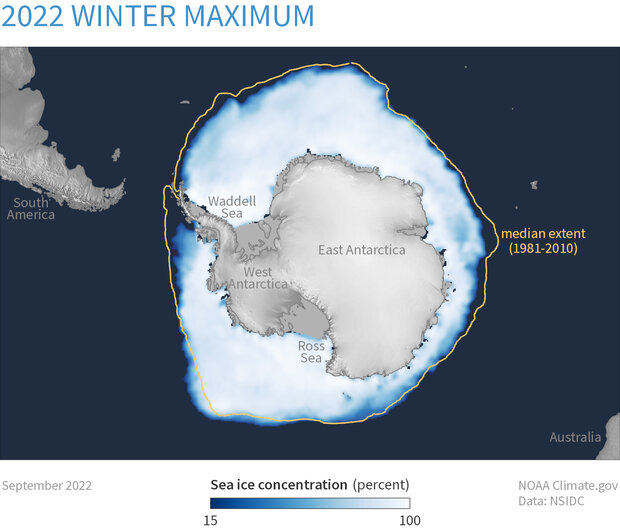
\includegraphics[width=\linewidth]{Figures/LiteratureReview/AntarcticClimate/seaIceExtentWinter2022.png} 
 		%\caption{Original Image}
	\end{subfigure}
	\hfill
	\begin{subfigure}[t]{.48\linewidth}
        \centering
		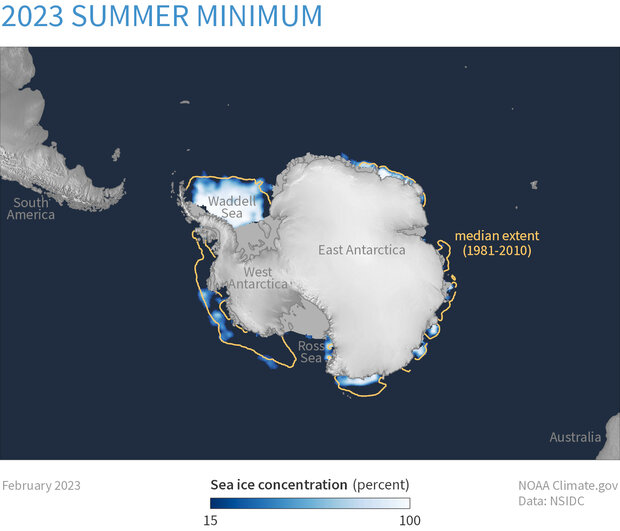
\includegraphics[width=\linewidth]{Figures/LiteratureReview/AntarcticClimate/seaIceExtentSummer2023.png} 
 		%\caption{Rotated Image \label{fig:dataRotate}}
	\end{subfigure}
    \caption{Comparison of sea ice extent in Antarctica between the winter of 2022 and summer of 2023. Taken from \cite{Scott2023}}
    \label{fig:litReview.antarcticClimate.seaIceExtent2022}
\end{figure}

%The maximum and minimum of this sea ice extent can vary year-on-year, and over the past 35 years, Antarctic sea ice extent has been observed to have slightly increased over each decade \cite{Comiso2017,Maksym2012,Simmonds2015}. This observation disagrees with the predictive models applied to model the Antarctic sea ice extent. Simmons investigated the application of \ac{cmip5}\footnote{\acs{cmip5}, which forms part of the \ac{cmip}, serves as a standard experimental framework designed to examine the output of coupled atmosphere-ocean general circulation models. This approach allows for the evaluation of a climate model's strengths and weaknesses when analysing climate variability and change. An overview of \acs{cmip5} can be found in the following paper by Taylor \cite{Taylor2012}.} models in Antarctica \cite{Simmonds2015} and discovered that these models perform well when analysing sea ice extent over 35 years in the Arctic \cite{Simmonds2015}, however, applying these models to Antarctica results in a decrease in sea ice extent being predicted. This is in direct opposition to the observations made in \cite{Comiso2017,Maksym2012}.


The maximum and minimum extents of sea ice can vary from year to year. Over the past 35 years,  a slight increase in Antarctic sea ice extent each decade has been observed \cite{Comiso2017,Maksym2012,Simmonds2015}. However, these observations contrast with predictive models used to estimate the Antarctic sea ice extent. Simmons \cite{Simmonds2015} examined the application of \ac{cmip5}\footnote{\acs{cmip5}, which forms part of the \ac{cmip}, serves as a standard experimental framework designed to examine the output of coupled atmosphere-ocean general circulation models. This approach allows for the evaluation of a climate model's strengths and weaknesses when analysing climate variability and change. An overview of \acs{cmip5} can be found in the following paper by Taylor \cite{Taylor2012}.} models in Antarctica. Simmons found that these models perform well in analysing Arctic sea ice extent over a 35-year period. However, when applied to Antarctica, these models predict a decrease in sea ice extent, contrary to the observations made in \cite{Comiso2017,Maksym2012}.

%Simmonds suggests that the discrepancies between the model outputs of the Arctic and the Antarctic can be attributed to natural variability \cite{Simmonds2015}. Simmonds also argues that, due to the period of study (35 years), the natural variability is less of an issue to the incorrect simulation outputs. Simmonds rather suggests that the differences can be attributed to the physics of the models; due to the fact that the \acs{cmip5} models work well when simulating Arctic ice, but poorly for Antarctic sea ice \cite{Simmonds2015}. This idea is confirmed by Maksym et al. due to the fact that pancake ice is not yet included in these types of models \cite{Maksym2012}. Pancake ice is an important part of the \acs{miz}, as well as a key process in sea ice-ocean interactions, and is discussed in the following sub-sections.

Simmonds suggests that the discrepancies between the model outputs of the Arctic and the Antarctic can be attributed to natural variability \cite{Simmonds2015}. He also argues that, given the 35-year study period, natural variability has less impact on the incorrect simulation outputs. Instead, Simmonds proposes that the differences can be attributed to the physics of the models. This is supported by the fact that the \acs{cmip5} models perform well in simulating Arctic ice but poorly in simulating Antarctic sea ice \cite{Simmonds2015}. This idea confirms the work of Maksym et al. \cite{Maksym2012}, as pancake ice, a significant component of the \acs{miz} and a key factor in sea ice-ocean interactions, is not yet considered in these models. The importance of pancake ice is discussed in the following sub-sections.

%Maksym et al. build on this idea that the physics of the sea ice models used in the Arctic will not translate to the Antarctic by introducing the differences between the two polar regions. The main differences can be attributed to the geography, sea-ice growth and decay, climate interactions, and ice-ocean interactions \cite{Maksym2012}. In terms of geography, the sea ice in the Arctic is landlocked by the Eurasian and North American continents \cite{Maksym2012,Parkinson2004} and is much more protected than sea ice in Antarctica, which is exposed to the \acs{so}. This means that sea ice in the Arctic is perennial\footnote{Perennial ice refers to ice packs that last more than one year and do not melt during the summer months}, whereas sea ice in the Antarctic is seasonal. As previously mentioned, the range of the sea ice extent in Antarctica is 1.5 times the extent of the Arctic \cite{Thomas2017}. In terms of climate interactions, the \acs{so} has extremely strong westerly winds, which results in large waves and frequent storms \cite{Maksym2012}. These westerly winds have caused the sea ice to extend further north\footnote{This is due to the fact that ice drifts to the left of the westerly winds due to a mechanism known as Ekman transport \cite{Maksym2012}} and increases the sea ice extent, which exposes sea ice to warmer temperatures \cite{Parkinson2004,Maksym2012}. The roughness and vastness of the \acs{so} are responsible for the difference in ice-ocean interactions between Arctic and Antarctic sea ice \cite{Parkinson2004} and is a dynamic system that is constantly in motion \cite{Maksym2012}. These mechanisms are discussed further in the following sub-sections, as well as the theory chapter.

Maksym et al. \cite{Maksym2012} build upon the idea that the physics of sea ice models used in the Arctic may not be directly applicable to the Antarctic. They introduce the distinctions between these two polar regions, highlighting key differences. The main disparities can be attributed to geographical factors, sea ice growth and decay patterns, climate interactions, and ice-ocean dynamics. In terms of geography, Arctic sea ice is enclosed by the Eurasian and North American continents \cite{Maksym2012, Parkinson2004}, affording it greater protection compared to the more exposed Antarctic sea ice, which interacts with the \acs{so}. Consequently, Arctic sea ice is considered perennial\footnote{Perennial ice refers to ice packs that persist for more than one year and do not melt during the summer months.}, whereas Antarctic sea ice is seasonal. As mentioned earlier, the extent of sea ice in Antarctica is 1.5 times greater than that of the Arctic \cite{Thomas2017Chap8}. Regarding climate interactions, the \acs{so} experiences strong westerly winds, resulting in substantial waves and frequent storms \cite{Maksym2012}. These prevailing westerly winds drive the sea ice northward\footnote{This is due to the ice being pushed to the left of the westerly winds through a mechanism known as Ekman transport \cite{Maksym2012}.}, expanding the sea ice coverage and consequently exposing it to warmer temperatures \cite{Parkinson2004, Maksym2012}. The roughness and vastness of the \acs{so} account for the distinctions in ice-ocean interactions between Arctic and Antarctic sea ice \cite{Parkinson2004}, which constitutes a dynamic system characterised by constant motion \cite{Maksym2012}.

%From the above literature, it can be seen that a large scientific effort is required to create accurate predictive models of Antarctica, rather than trying to apply predictive models built for an Arctic environment. The harshness of the Antarctic climate has meant that, particularly during winter, field measurements of the spatial distribution of sea ice in Antarctica are lacking \cite{Maksym2012}. Gherardi et al., and Kennicut et al. both agree that improved remote sensing techniques need to be implemented to monitor the extent of sea ice in Antarctica \cite{Gherardi2015,Kennicut2019}. Maksym et al. go one step further, by hypothesising that the thickness of sea ice may be more sensitive to climate variability than extent \cite{Maksym2012}, which explains the increase in melt, but also the increase in extent discussed. However, in-situ measurements are required to measure ice thickness in Antarctica instead of remote sensing techniques - as employed in the Arctic \cite{Gherardi2015,Thomas2017}. Maksym et al. argue that if researchers lack the ability to evaluate models of Antarctic sea ice, the confidence in the accuracy of projections will be brought into question, as models cannot capture the current state of sea ice in Antarctica \cite{Maksym2012}. This shows the need for the development of a pipeline to extract sea ice parameters in Antarctica, however, the issues discussed above cannot be mitigated. The differences between Arctic and Antarctic models are the presence of the \acs{miz} and pancake ice in this region, which is a key process in the sea ice-ocean interactions \cite{Maksym2012}. 

From the literature above, it is evident that significant scientific endeavour is necessary to create accurate predictive models of Antarctic sea ice, rather than attempting to apply predictive models built for an Arctic environment. The severity of the Antarctic climate has resulted in a lack of field measurements, particularly during winter, regarding the spatial distribution of sea ice in Antarctica \cite{Maksym2012}. Both Gherardi et al. \cite{Gherardi2015} and Kennicut et al. \cite{Kennicut2019} agree that implementing improved remote sensing techniques is essential to monitor the extent of sea ice in Antarctica. Taking this further, Maksym et al. \cite{Maksym2012} hypothesise that the thickness of sea ice may be more responsive to climate variability than sea ice extent. This not only explains the increase in melt but also the discussed increase in extent. However, measuring ice thickness in Antarctica requires in-situ measurements instead of the remote sensing techniques employed in the Arctic \cite{Gherardi2015, Thomas2017Chap8}.

Maksym et al. \cite{Maksym2012} argue that the inability to evaluate models of Antarctic sea ice by researchers raises questions about the accuracy of projections. This is because models fail to capture the current state of sea ice in Antarctica. This highlights the necessity for developing a pipeline to extract sea ice parameters in Antarctica. Nonetheless, the aforementioned issues cannot be easily mitigated. Notably, the differences between Arctic and Antarctic models include the interactions between the \acs{miz} and the \acs{so}, and pancake ice, which play a crucial role in sea ice-ocean interactions in Antarctica.


\subsection{Marginal Ice Zone} \label{subsec:litReview.antarctica.miz}
% Explain ice-ocean interaction (Link to theory section - only provide overview!)
% Chapter 8 of Sea-Ice
%The \ac{miz} in Antarctica is defined as the area that is close enough to the \ac{so} to be affected by its presence \cite{Wadhams1986}. The \ac{miz} in Antarctica is a dynamic system due to the prevalence of strong westerly winds and storms in the ice-free zones of the \acs{so} \cite{Massom2010, Brouwer2022, Maksym2012}, allowing for greater freedom of movement. The \acs{miz} is a region where sea-ice-ocean-atmosphere interactions are closely linked \cite{Wadhams1986, Vichi2019}. As discussed, the climate of Antarctica and the \acs{so} is incredibly harsh. The sea ice in the Antarctic \acs{miz} plays an important role in the interconnected global climate and being able to understand \acs{miz} dynamics allows the response of Antarctic sea ice, as well as the impacts of this, to climate change and variability to be understood \cite{Brouwer2022}. The \acs{miz} is controlled by a variety of processes, which are introduced in the following sub-section and discussed in more detail in the theoretical development chapter.

The \ac{miz} in Antarctica is defined as the area that is close enough to the \ac{so} to be affected by its presence \cite{Wadhams1986}. This region experiences dynamic conditions due to the prevalence of strong westerly winds and storms in the ice-free zones of the \acs{so} \cite{Massom2010, Brouwer2022, Maksym2012}, allowing for greater freedom of movement. The \acs{miz} is a region where sea-ice-ocean-atmosphere interactions are closely linked \cite{Wadhams1986, Vichi2019}. As discussed, the climate of Antarctica and the \acs{so} is incredibly harsh. Sea ice within the Antarctic \acs{miz} plays a crucial role in the global climate system \cite{Parkinson2004}, and comprehending the dynamics of the MIZ contributes to understanding the responses of Antarctic sea ice to climate change and variability, along with its associated impacts \cite{Brouwer2022}. The \acs{miz} is influenced by a variety of processes, which will be introduced in the following subsection.

The \acs{miz} plays a critical role in the global climate by forming a seasonal, insulating "skin" atop the \acs{so}. Due to the characteristics of sea ice, its high albedo reflects solar radiation and serves as an effective insulator \cite{Parkinson2004, Massom2010}. Consequently, sea ice within the \acs{miz} helps regulate \acs{so} temperatures by limiting heat exchanges between the \acs{so} and the atmosphere \cite{Parkinson2004}. Moreover, the presence of sea ice over the \acs{so} increases the salinity and density of the \acs{so} due to the seasonal formation of sea ice \cite{Massom2010, Parkinson2004}. This aspect is crucial for global ocean circulation \cite{Thomas2017Chap8}. The increased density beneath the sea ice in the \acs{miz} leads to overturning and the formation of bottom water\footnote{The resulting \ac{aabw} is the coldest in the world and has far-reaching climatic impacts. More information on bottom water formation, as well as its importance to the global climate, can be found in \cite{Gordon2001,Thomas2017Chap8,Jacobs2004}.} \cite{Parkinson2004}.

%Further to the sea ice-atmosphere and ocean interactions discussed, the most important aspect of the \acs{miz}, in the context of this project, is the way in which the Antarctic \acs{miz} interacts with wave motion from the \acs{so} as well as the features of the \acs{miz} which regulate this process. Brouwer et al. summarise this process nicely, by saying that the wave-ice interactions are mutual. Brouwer et al. state that the waves, which propagate through the \acs{miz}, alter the properties of the sea ice, however, when doing so, the wave amplitude is attenuated through the energy required to alter the sea ice properties \cite{Brouwer2022}. The way in which sea ice in the \acs{miz} attenuates waves is similar to that of a low-pass filter \cite{Brouwer2022}. This means that waves with a higher frequency are attenuated - where the rate depends on the physical characteristics of the sea ice, such as floe size, thickness and concentration \cite{Squire2020,Montiel2022}.

In addition to the discussions on sea ice-atmosphere and ocean interactions, the most crucial aspect of the \acs{miz} in the context of this project is its interaction with wave motion from the \acs{so}, as well as the characteristics of the \acs{miz} that regulate this process. Brouwer et al. \cite{Brouwer2022} summarise this phenomenon by stating that wave-ice interactions are mutual. According to Brouwer et al., the waves propagating through the \acs{miz} modify the properties of the sea ice. However, during this process, the wave amplitude is attenuated due to the energy required to alter the sea ice properties. The manner in which sea ice within the \acs{miz} attenuates waves is comparable to that of a low-pass filter. This implies that waves with higher frequencies are attenuated, with the rate of attenuation depending on the physical characteristics of the sea ice, such as floe size, thickness, and concentration \cite{Squire2020, Montiel2022}.

%Stammerjohn et al. state that these sea ice-ocean interactions are important to understand as they impact the sea ice features and distribution, which, in turn, impacts the regional, polar climate and global climate \cite{Stammerjohn2012}. This impact has been observed by Asplin et al. and Stopa et al., albeit in the Arctic \acs{miz}, whereby surface gravity waves, with a long period\footnote{The dynamics of ocean waves, as well as the different types for shallow and deep water, are explained quantitatively in the theoretical development section of this report. For the readers' interest, more information can be found in \cite{Holthuijsen2007}.}, have penetrated hundreds of kilometres into the Arctic \acs{miz} before being completely attenuated \cite{Asplin2012,Stopa2018}. This is an important observation, even for the Antarctic \acs{miz}, as long-period and high-amplitude waves occur frequently due to the harshness of the \acs{so} \cite{Young2020}, and the way in which these waves penetrate and become attenuated in the Antarctic \acs{miz} needs to be understood \cite{Alberello2021,Weeks2011}.

Stammerjohn et al. \cite{Stammerjohn2012} state that understanding sea ice-ocean interactions is crucial, as they influence sea ice features and distribution. These, in turn, affect both regional and polar climates, as well as the global climate. This impact has been observed in the Arctic \acs{miz} by Asplin et al. \cite{Asplin2012} and Stopa et al. \cite{Stopa2018} These researchers noted the penetration of long-period surface gravity waves\footnote{For an in-depth, quantitative explanation of ocean wave dynamics, including various types in shallow and deep waters, refer to Chapter \ref{chap:theory} in this report. Additional information can be found in \cite{Holthuijsen2007}.}, reaching hundreds of kilometres into the Arctic \acs{miz} before being completely attenuated \cite{Asplin2012,Stopa2018}. This observation holds significance not only for the Arctic but also for the Antarctic \acs{miz}, where long-period and high-amplitude waves occur frequently due to the harshness of the \acs{so} \cite{Young2020}. It is imperative to understand how these waves penetrate and are attenuated within the Antarctic \acs{miz} \cite{Alberello2021}.

%This understanding is required because currently the \acs{miz} is viewed using remote sensing techniques via passive satellite technology to define the \acs{miz} using \ac{sic}. The ice edge is defined as 15\,\% \acs{sic}, whereas close ice is defined as 80\,\% \acs{sic} \cite{WMO2014}. However, using this metric to define the \acs{miz}, is not ideal, as it does not take into account wave interactions with the sea ice \cite{Brouwer2022}. According to Vichi, the use of \acs{sic} to understand the \acs{miz} characteristics in the Arctic is effective, however, applying this to the Antarctic \acs{miz} is not as reliable \cite{Vichi2021}. Vichi states that this is due to increased wave penetration and sea ice drift \cite{Vichi2019,Vichi2021}. Instead of using \acs{sic}, Vichi proposes a different approach to defining the \acs{miz}. Vichi's proposal is one that uses the statistical properties of \acs{sic} in the \acs{miz}, as well as the spatial and temporal variability of the \acs{sic} in the \acs{miz} \cite{Vichi2021}. This will allow the effects of different ice types, as well as wave action from the \acs{so} to be considered. 

This understanding is required because the current definition of the \acs{miz} relies on remote sensing techniques employing passive satellite technology to define the \acs{miz} through the use of \ac{sic}. The ice edge is conventionally defined as having 15\,\% \acs{sic}, while compact ice is characterized by 80\,\% \acs{sic} \cite{WMO2014}. However, employing this metric to define the Antarctic \acs{miz} is inefficient, as it overlooks wave interactions with the sea ice \cite{Brouwer2022,Vichi2021}. According to Vichi \cite{Vichi2021}, the use of \acs{sic} to comprehend \acs{miz} characteristics in the Arctic is effective; whilst, its application to the Antarctic \acs{miz} lacks reliability. Vichi \cite{Vichi2019,Vichi2021} asserts that this discrepancy is attributed to heightened wave penetration and sea ice drift. In place of \acs{sic}, Vichi proposes an alternate approach to defining the \acs{miz}. Vichi's recommendation involves utilising the statistical properties of \acs{sic} within the \acs{miz}, alongside the spatial and temporal variability of \acs{sic} in the same zone \cite{Vichi2021}. This approach will enable the consideration of distinct ice types, along with wave activity from the \acs{so} \cite{Vichi2021}.


\subsection{Pancake Ice} \label{subsec:litReview.antarctica.pancakeIce}
% Importance of pancake ice
% Mention frazil ice
% WHY pancake ice forms in the Antarctic and is important in it
% Yearly life cycle of pancake ice

As noted by Maksym et al. \cite{Maksym2012}, one of the key processes in the Antarctic \acs{miz} is pancake ice formation. Given the vastness of the \acs{so} and the prevalence of the \acs{miz} in Antarctica, the existence of waves within the \ac{miz} significantly influences the types of ice found within the \acs{miz} \cite{Brouwer2022}. This section provides a brief introduction to the formation and life cycle of pancake ice, followed by an exploration of its significance in shaping the Antarctic climate. Furthermore, this section introduces its crucial role in Antarctic sea ice modelling.

The formation of pancake ice in the \acs{miz} is poorly understood \cite{Doble2003}. In summer, large ice floes make up the \acs{miz}, whereas, in winter the \acs{miz} is made up of millions of smaller pancake ice floes \cite{Alberello2019,Alberello2021b} The presence of the rough sea surface means that the formation of ice is not allowed to settle into a fully formed ice sheet. Rather, when sea ice begins to form in the Antarctic in winter, it begins to create a suspension of crystals known as frazil ice \cite{Doble2003,Wadhams1999}. Over time, these frazil crystals converge, due to roughened seas, and collect to form small cakes \cite{Doble2003,Dierking2013} Initially, these small cakes are referred to as "dollar pancakes" \cite{Wadhams1999}, with a diameter of approximately 2-3\,cm and a thickness of only a few millimetres \cite{Doble2003,Wadhams1999}. At greater distances from the ice edge in the \acs{miz}, these dollar pancakes can fuse together due to wave attenuation, forming larger pancakes with a diameter of up to 5\,m and a thickness of approximately 50\,cm \cite{Wadhams1999,Aulicino2014,Doble2003}. In 2019, Alberello et al. \cite{Alberello2019} found that approximately 50\,\% of the observed sea ice area was made up of pancake ice floes ranging from 2.3 - 4m in diameter. Only further into the \acs{miz}, at approximately 270\,km \cite{Wadhams1987}, where wave action has been attenuated even more, can these pancakes freeze together to form an ice sheet known as consolidated pancake ice. Once consolidated pancake ice is formed, thickening of these consolidated pancakes occurs to form pack ice \cite{Doble2003}. 

% How it influences climate - why the ice plays a vital role 

%Pancake ice formation is key to pack ice formation in Antarctica \cite{Clarke1984,Lange1991} and as discussed in Section \ref{subsec:litReview.antarctica.miz}, the importance of sea ice is critical to the global climate and understanding the processes behind the formation, evolution and distribution of sea ice, particularly pancake ice, is vital to explain the geophysical interactions in the polar regions, particularly the \acs{miz} \cite{DeCarolis2002}. Firstly, pancake ice is important in the production of a fertile winter ecosystem due to its ability for increased algal growth and shelter for krill due to its rafted bottom which provides a large surface area \cite{Wadhams2002}. Secondly, the gravity-induced drainage of brine after pancake formation is responsible for regulating the salinity of the \acs{so}, as well as previously discussed, the high albedo of sea ice provides an insulating layer on top of the \acs{so}, and helps in regulating \acs{so} temperatures \cite{Doble2003}.

Pancake ice formation is key to pack ice formation in Antarctica \cite{Clarke1984,Lange1991}. As discussed in Section \ref{subsec:litReview.antarctica.miz}, the importance of sea ice is critical to the global climate. Understanding the processes behind the formation, evolution, and distribution of sea ice, particularly pancake ice, is vital for explaining the geophysical interactions in the polar regions, especially the \acs{miz} \cite{DeCarolis2002}.

Firstly, pancake ice plays a significant role in the production of a fertile winter ecosystem due to its ability to promote increased algal growth and provide a shelter for krill as its rafted bottom creates a large surface area \cite{Wadhams2002}. Secondly, the gravity-induced drainage of brine after pancake formation helps regulate the salinity of the \acs{so}. Additionally, as previously discussed, the high albedo of sea ice serves as an insulating layer atop the \acs{so} and aids in regulating its temperatures \cite{Doble2003}.

%The modelling of pancake ice is not particularly well understood and is currently being incorporated into existing sea ice models \cite{Alberello2019}. The understanding of pancake ice, particularly its impact on wave attenuation is important as according to both Doble et al. and Alberello et al. \cite{Alberello2019,Doble2015}, increased open water area present in the Arctic is causing an increased presence of pancake ice in the region. This is important, as the models which currently exist for this region, are slowly becoming less accurate due to these changes in the region's sea ice composition \cite{Doble2015}.

The modelling of pancake ice is not particularly well understood and is currently being incorporated into existing sea ice models \cite{Alberello2019}. The understanding of pancake ice, particularly its impact on wave attenuation, is important, as indicated by both Doble et al. \cite{Doble2015} and Alberello et al. \cite{Alberello2019}. The increased open water area in the Arctic is leading to a greater presence of pancake ice in the region \cite{Alberello2019,Doble2015}. This is significant because the existing models for this region are gradually decreasing in accuracy due to the changing composition of the sea ice in the region. In order to properly model the region, sea ice models including properly characterised pancake ice floes are required \cite{Doble2015}.


%====================================================
\section{Characterisation of Sea Ice}
\label{sec:litReview.seaIceCharac}
% Existing technology and work (not necessarily SAR)
% Chapter 9 of Sea-Ice
% Importance of ocean waves in modelling (Holthuijsen)

This section will introduce the existing technologies and research that have been employed to characterise sea ice in both the Arctic and Antarctic regions. These methods will be briefly examined, focusing on their advantages and disadvantages in implementation. Subsequently, the technique of sea ice characterisation using \acs{sar} will be introduced in the subsequent section. The importance of ocean waves in modelling will also be discussed. %As mentioned earlier, the differentiation between Arctic and Antarctic sea ice modelling will be emphasised in relation to these technologies.

While in-situ measurements are the most practical method for determining sea ice characteristics, as discussed in Section \ref{sec:litReview.antarcticClimate}, a vast expanse of the Antarctic \acs{miz} is inaccessible in winter due to the formation of thick sea ice that cannot be navigated, even by ice-breaking ships \cite{Maksym2012}. Thus, remote sensing techniques\footnote{Spreen and Kern \cite{Thomas2017Chap9} define remote sensing as any form of data acquisition without the need for physical contact or measurement.} need to be implemented to monitor the Antarctic \acs{miz} year-round due to the harshness of the region \cite{Kennicut2019, Maksym2012}. Since the scope of this project revolves around \acs{sar} - a remote sensing technique in itself - this section will focus on remote sensing techniques for sea ice characterisation.

Remote sensing techniques rely on the \ac{em} spectrum and satellite remote sensing of sea ice is conducted in multiple parts of the \acs{em} spectrum \cite{Thomas2017Chap9}. Different frequency ranges of the spectrum are used, and the reflected intensity measured by the sensors depends on the ability of sea ice, water, and snow to emit \acs{em} radiation. The ability of sea ice to emit this \acs{em} radiation is determined by its geophysical properties, such as salinity, roughness, and air content \cite{Thomas2017Chap9}. These geophysical properties can be inferred from the received intensity at the sensor. The \acs{em} radiation emitted back by sea ice can originate from either a passive source, such as the sun, or an active source, such as a \acs{sar} transmitter. The following sub-sections introduce three different remote sensing techniques which operate at different frequencies in the \acs{em} spectrum.

\subsection{Microwave radiometry and scatterometry} \label{subsec:litReview.seaIceCharac.radiometry}

For optimal sea ice microwave remote sensing, frequencies of less than 10\,GHz are used. While higher frequencies result in better spatial resolution, the influence of atmospheric conditions increases. Thus, microwave remote sensing of sea ice always involves a trade-off between atmospheric influence and spatial resolution \cite{Thomas2017Chap9}.

Microwave radiometry has been employed to measure sea ice extent and types. For sea ice extent determination, both microwave radiometry and scatterometry have been utilised. To gauge sea ice extent through microwave radiometry, the brightness temperature, denoted as $T_{B}$, plays a significant role. $T_{B}$ is predominantly influenced by the emissivity\footnote{Emissivity, a material-specific property, is a function of the dielectric properties of the material \cite{Thomas2017Chap9}.} of the sea ice or sea surface. The distinction in $T_{B}$ between the sea ice and sea is utilised to define the sea ice extent. However, this approach encounters limitations when the sea surface becomes roughened by wind, leading to an increase in the emissivity of the sea's surface. Consequently, the $T_{B}$ of the sea surface reaches a similar level to that of the sea ice \cite{Thomas2017Chap9}. In the context of Antarctica, this issue arises due to the rough nature of the \acs{so}, potentially interfering with the differentiation between sea ice and the ocean surface. 

Scatterometry can also be used to determine sea ice extent. The difference in radar backscatter\footnote{Backscatter is the reflection of a signal back towards its source.} between uncovered open water and sea ice enables the detection of an ice-covered region \cite{Thomas2017Chap9}. Rivas et al. \cite{Rivas2018} discovered that scatterometry is more accurate than microwave radiometry in determining sea ice extent, especially when the edge of the extent is composed of frazil ice.

The backscatter of different ice types differs depending on the ice's salinity, density, roughness, temperature, and snow coverage \cite{Thomas2017Chap9}. This differentiation allows the identification of various types of ice within a sea ice region based on the received backscatter intensity. Dierking \cite{Dierking2001} found that pancake ice exhibits higher radar backscatter compared to other ice types due to its increased surface roughness and the presence of numerous edges. This observation has been confirmed by Lange and Eicken \cite{Lange1991} through their study of higher radar backscatter in the Antarctic \acs{miz}.

\subsection{Altimetry} \label{subsec:litReview.seaIceCharac.altimetry}

Altimeters measure the time taken by an \acs{em} signal to be transmitted, reflected off the Earth's surface, and received. From this, the distance can be calculated. Laser and radar altimeters can be used to measure sea ice thickness. However, instead of directly measuring the thickness, these altimeters measure the sea ice freeboard\footnote{Freeboard is defined by Ricker et al. \cite{Ricker2015} as the height of sea ice above the local sea level.}, and infer the thickness from the sea surface height. To extract the surface elevation, the satellite's position in space needs to be known with centimetre accuracy \cite{Thomas2017Chap9}.

To calculate sea ice thickness, both the freeboard and sea surface height need to be determined by the altimeter. One issue with sea surface height determination is the need to access uncovered ocean to act as a reference point \cite{Thomas2017Chap9}. In order to convert freeboard height to sea ice thickness, the density and snow depths need to be known. Ricker et al. \cite{Ricker2015} show that the origin of the return signal of the altimeter cannot always be known with certainty and state that snow cover is not negligible in determining distances due to the fact that the signals do not penetrate the snow completely, thus creating bias in measurements. Given that Antarctica experiences some of the highest snowfall rates in the world \cite{Maksym2012}, this method will be unable to be implemented without the aid of in-situ measurements of snow depth \cite{Ricker2015}. Spreen and Kern \cite{Thomas2017Chap9} explain that improved retrieval methods using altimeters need to be implemented to overcome this.

\subsection{Optical and Thermal infrared imaging} \label{subsec:litReview.seaIceCharac.opticalThermal}

Optical and thermal infrared imaging techniques rely on the fact that sea ice reflects solar radiation more than open, uncovered water \cite{Thomas2017Chap9}. Optical imagery has been used to measure \acs{sic} \cite{Emery1994} as well as thickness. Thermal imaging is useful, as sensors can measure the surface temperature, $T_{\text{surface}}$, of sea ice \cite{Thomas2017Chap9}.

The average sea ice albedo is greater than 0.6, compared to the low albedo of water, which is 0.07. Brandt et al. \cite{Brandt2005} found that the albedo of ice increased with thickness \cite{Thomas2017Chap9}, allowing these techniques to be used for measuring ice thickness. To measure the surface albedo using a satellite, a sensor capable of measuring surface reflectance needs to be employed \cite{Thomas2017Chap9}.

The main disadvantage of this technology is its limitations. Both optical and thermal imaging technologies require daylight as well as clear sky conditions to capture the desired data. Clouds pose a significant challenge for both of these technologies. In the optical spectrum, clouds exhibit similar reflectivity to sea ice, and the infrared temperatures of the surface of sea ice and clouds are also similar \cite{Thomas2017Chap9}. These issues imply that while this technology has been utilised for parameter extraction of sea ice, it can only be applied within a narrow time frame determined by environmental conditions, preventing year-round coverage of Antarctica.

%====================================================
\section{Sea Ice Characterisation using SAR} 
\label{sec:litReview.sarCharac}
% Explain BRIEFLY what sar is and why it is used for sea ice characterisation
% Introduce section (Which satellites, as well as a brief overview of the inversion technique and its path to where we are now)
% What characteristics are important to the SAR process e.g. thickness for radar penetration and snow coverage for reflection
%% - Discuss differences in reflectiveness of different elements

[I need to beef this out still - I want to use the following sources, \cite{Dierking2013,Zakhvatkina2019,Thomas2017Chap9} to introduce the process followed by the \acs{irea} and discuss which \acs{sar} characteristics have been found to be important to the parameter extraction process of pancake ice.]

The main disadvantage of the remote sensing methods mentioned above is the low spatial resolution. \acs{sar} overcomes this by using the motion of a satellite to synthetically increase the size of the antenna \cite{Thomas2017Chap9}. \acs{sar} has been used to determine sea ice type through differences in radar backscatter. 

\subsection{SAR Satellites}
\label{subsec:litReview.sarCharac.satellites}
% Discuss the satellite technology needed to implement sar - specifically for polar regions
% TerraSAR-X, Sentinel-1, CosmosSkyMet, and others
% Sentinel-1 TODO

Due to the nature of orbits around the planet\footnote{For an orbit to capture polar regions, it needs to have a 90\,$^{\circ}$ inclination orbit \cite{PolarOrbitNasa}}, only specific \acs{sar} satellites can effectively monitor the polar regions \cite{Thomas2017Chap9}. These commonly used satellites are outlined in Table \ref{tab:litReview.sarCharac.satellites.commonlyUsed}, along with key features of interest. The meaning and significance of these features will be expanded on and explained in Chapter \ref{chap:theory}.

\begin{table}[H]
\resizebox{\textwidth}{!}{%
\begin{tabular}{|l|c|c|c|c|c|c|c|c|}
\hline
\textbf{Name} & \textbf{\begin{tabular}[c]{@{}c@{}}Frequency\\ (GHz)\end{tabular}} & \textbf{\begin{tabular}[c]{@{}c@{}}Frequency\\ Band\end{tabular}} & \textbf{\begin{tabular}[c]{@{}c@{}}Resolution\\ (m)\end{tabular}} & \textbf{\begin{tabular}[c]{@{}c@{}}Swath\\ (km)\end{tabular}} & \textbf{\begin{tabular}[c]{@{}c@{}}Incidence Angle\\ ($^\circ$)\end{tabular}} & \textbf{\begin{tabular}[c]{@{}c@{}}Inclination\\ ($^\circ$)\end{tabular}} & \textbf{Operational} & \textbf{Polarisation} \\ \hline
\textbf{ERS-1} and \textbf{2} & 5.3 & C & 30 & 100 & 20-26 & 98.5 & 1991-2011 & VV \\ \hline
\textbf{Envisat ASAR} & 5.3 & C & 30-1000 & 100-400 & 15-45 & 98.5 & 2002-2012 & Dual-polarimetric\footnote{Explain dual polarimetric polarisation} \\ \hline
\textbf{Radarsat-1} and \textbf{2} & 5.3/5.4 & C & 3-100 & 18-500 & 10-60 & 98.6 & 1995- & \begin{tabular}[c]{@{}c@{}}HH (RS-1)\\ Full\footnote{Explain full polarisation} (RS-2)\end{tabular} \\ \hline
\textbf{Sentinel-1} & 5.4 & C & 5-100 & 80-400 & 19-47 & 98.2 & 2014- & Full \\ \hline
\textbf{TerraSAR-X} & 9.6 & X & 1-40 & 5-200 & 15-60 & 97.4 & 2007- & Full \\ \hline
\textbf{ALOS-1} and \textbf{2 PALSAR} & 1.3 & L & 3-100 & 20-350 & 8-70 & 98.7 (AL-1), 97.9 (AL-2) & \begin{tabular}[c]{@{}c@{}}2006-2011 (AL-1)\\ 2014- (AL-2)\end{tabular} & Full \\ \hline
\textbf{COSMO-SkyMed} & 9.6 & X & 1-100 & 10-100 & 16-51 & 97.9 & 2007- & Dual-polarimetric \\ \hline
\end{tabular}}
\caption{Commonly used \acs{sar} sensors for sea ice research and a comparison of their important features. Adapted from \cite{Thomas2017Chap9}.}
\label{tab:litReview.sarCharac.satellites.commonlyUsed}
\end{table}

As per the scope of this project, data obtained from Sentinel-1 and TerraSAR-X will be used for pipeline development and testing. As such, these satellites will be investigated further in this subsection.

\subsubsection{Sentinel-1} \label{sybsubsec:litReview.sarCharac.satellites.sentinel}

%Sentinel-1 is the first of a series of operational satellites launched by the \ac{esa} as part of the \ac{gmes} - a European initiative to meet the Earth Observation needs of the European Union \cite{Attema2009}. The Sentinel-1 is a constellation of two \acs{sar} satellites that include both the Sentinel-1A and Sentinel-1B satellites, which were launched on April 3, 2014, and April 25, 2016, respectively \cite{Geudtner2014,Potin2019}. Sentinel-1 is equipped with an active phased array antenna operating at C-Band frequency \cite{Geudtner2014}, capable of functioning in various modes\footnote{These modes include Interferometric Wide Swath, Extra Wide Swath, StripMap, and Wave. All of these modes, except Wave, operate in dual polarization. More information on the Sentinel-1 imaging modes can be found in Figure 1 and Table 1 of \cite{Geudtner2014}.}. Sentinel-1 is capable of providing data to support multiple applications, however, the main application of interest is the ability to monitor sea ice zones which cover the Arctic and the Antarctic \cite{Attema2009,Geudtner2014}, as well as the open-source data policy \cite{Potin2019}.

Sentinel-1 is the first in a series of operational satellites launched by the \ac{esa} as part of the \ac{gmes} program - an initiative aimed at meeting the Earth Observation needs of the European Union \cite{Attema2009}. The Sentinel-1 constellation comprises two \acs{sar} satellites: \ac{s1a} and Sentinel-1B. These satellites were launched on April 3, 2014, and April 25, 2016, respectively \cite{Geudtner2014, Potin2019}. Equipped with an active phased array antenna operating at C-Band frequency, Sentinel-1 is capable of operating in various modes\footnote{These modes include \acf{iw}, \acf{ew}, \acf{sm}, and Wave. All these modes, except Wave, operate in dual polarisation. Further details on the Sentinel-1 imaging modes can be found in Figure 1 and Table 1 of \cite{Geudtner2014}.}. While Sentinel-1 serves multiple applications, its primary focus is on monitoring sea ice zones in the Arctic and Antarctic regions \cite{Attema2009, Geudtner2014}, in addition to operating on an open-source data policy \cite{Potin2019}.

This application is achieved through the orbit of Sentinel-1. Both \ac{s1a} and Sentinel-1B fly in the same orbital plane; however, they are phased by 180\,$^{\circ}$\footnote{This phased orbit of the constellation means that the satellites are on opposite sides of the Earth at any given time. More information can be found in \cite{Geudtner2014}.}. The mission is on a sun-synchronous orbit\footnote{Sun-synchronous orbits allow a satellite to cross the same latitude at the same solar time of day on each orbit \cite{Hulley2019}.} and has a 12-day orbit repeat cycle \cite{Torres2012}. To ensure a polar orbit, the satellites have an inclination angle of 98.2\,$^{\circ}$, as shown in Table \ref{tab:litReview.sarCharac.satellites.commonlyUsed}. The open-source policy of this mission is useful for this project, as Level 0, Level 1, and Level 2 data products\footnote{The differentiation between these data is discussed in the theoretical development chapter.} are available for download on the \href{https://scihub.copernicus.eu/dhus/#/home}{Sentinel Copernicus Open Hub} \cite{Potin2019}.

The global coverage of Sentinel-1 in\acf{iw} mode is depicted in Figure \ref{fig:litReview.sarCharac.satellites.sentinel.coverage}. The captures encompassing the Antarctic continent in Figure \ref{fig:litReview.sarCharac.satellites.sentinel.coverage} are of particular interest to this project. Garkusha and Hnatushenko \cite{Garkusha2020} utilised data from this region to compile a mosaic of the entire Antarctic coastline using Sentinel-1 \acs{sar} data. The coverage of the coastline is illustrated in Figure \ref{fig:litReview.sarCharac.satellites.sentinel.coverageCoast.sentinel}. To achieve complete coverage for the construction of this mosaic, Garkusha and Hnatushenko employed GRD data from 98 captures from Sentinel-1. This mosaic construction is illustrated in Figure \ref{fig:litReview.sarCharac.satellites.sentinel.coverageCoast.mosaic}.

\begin{figure}[H]
    \centering
    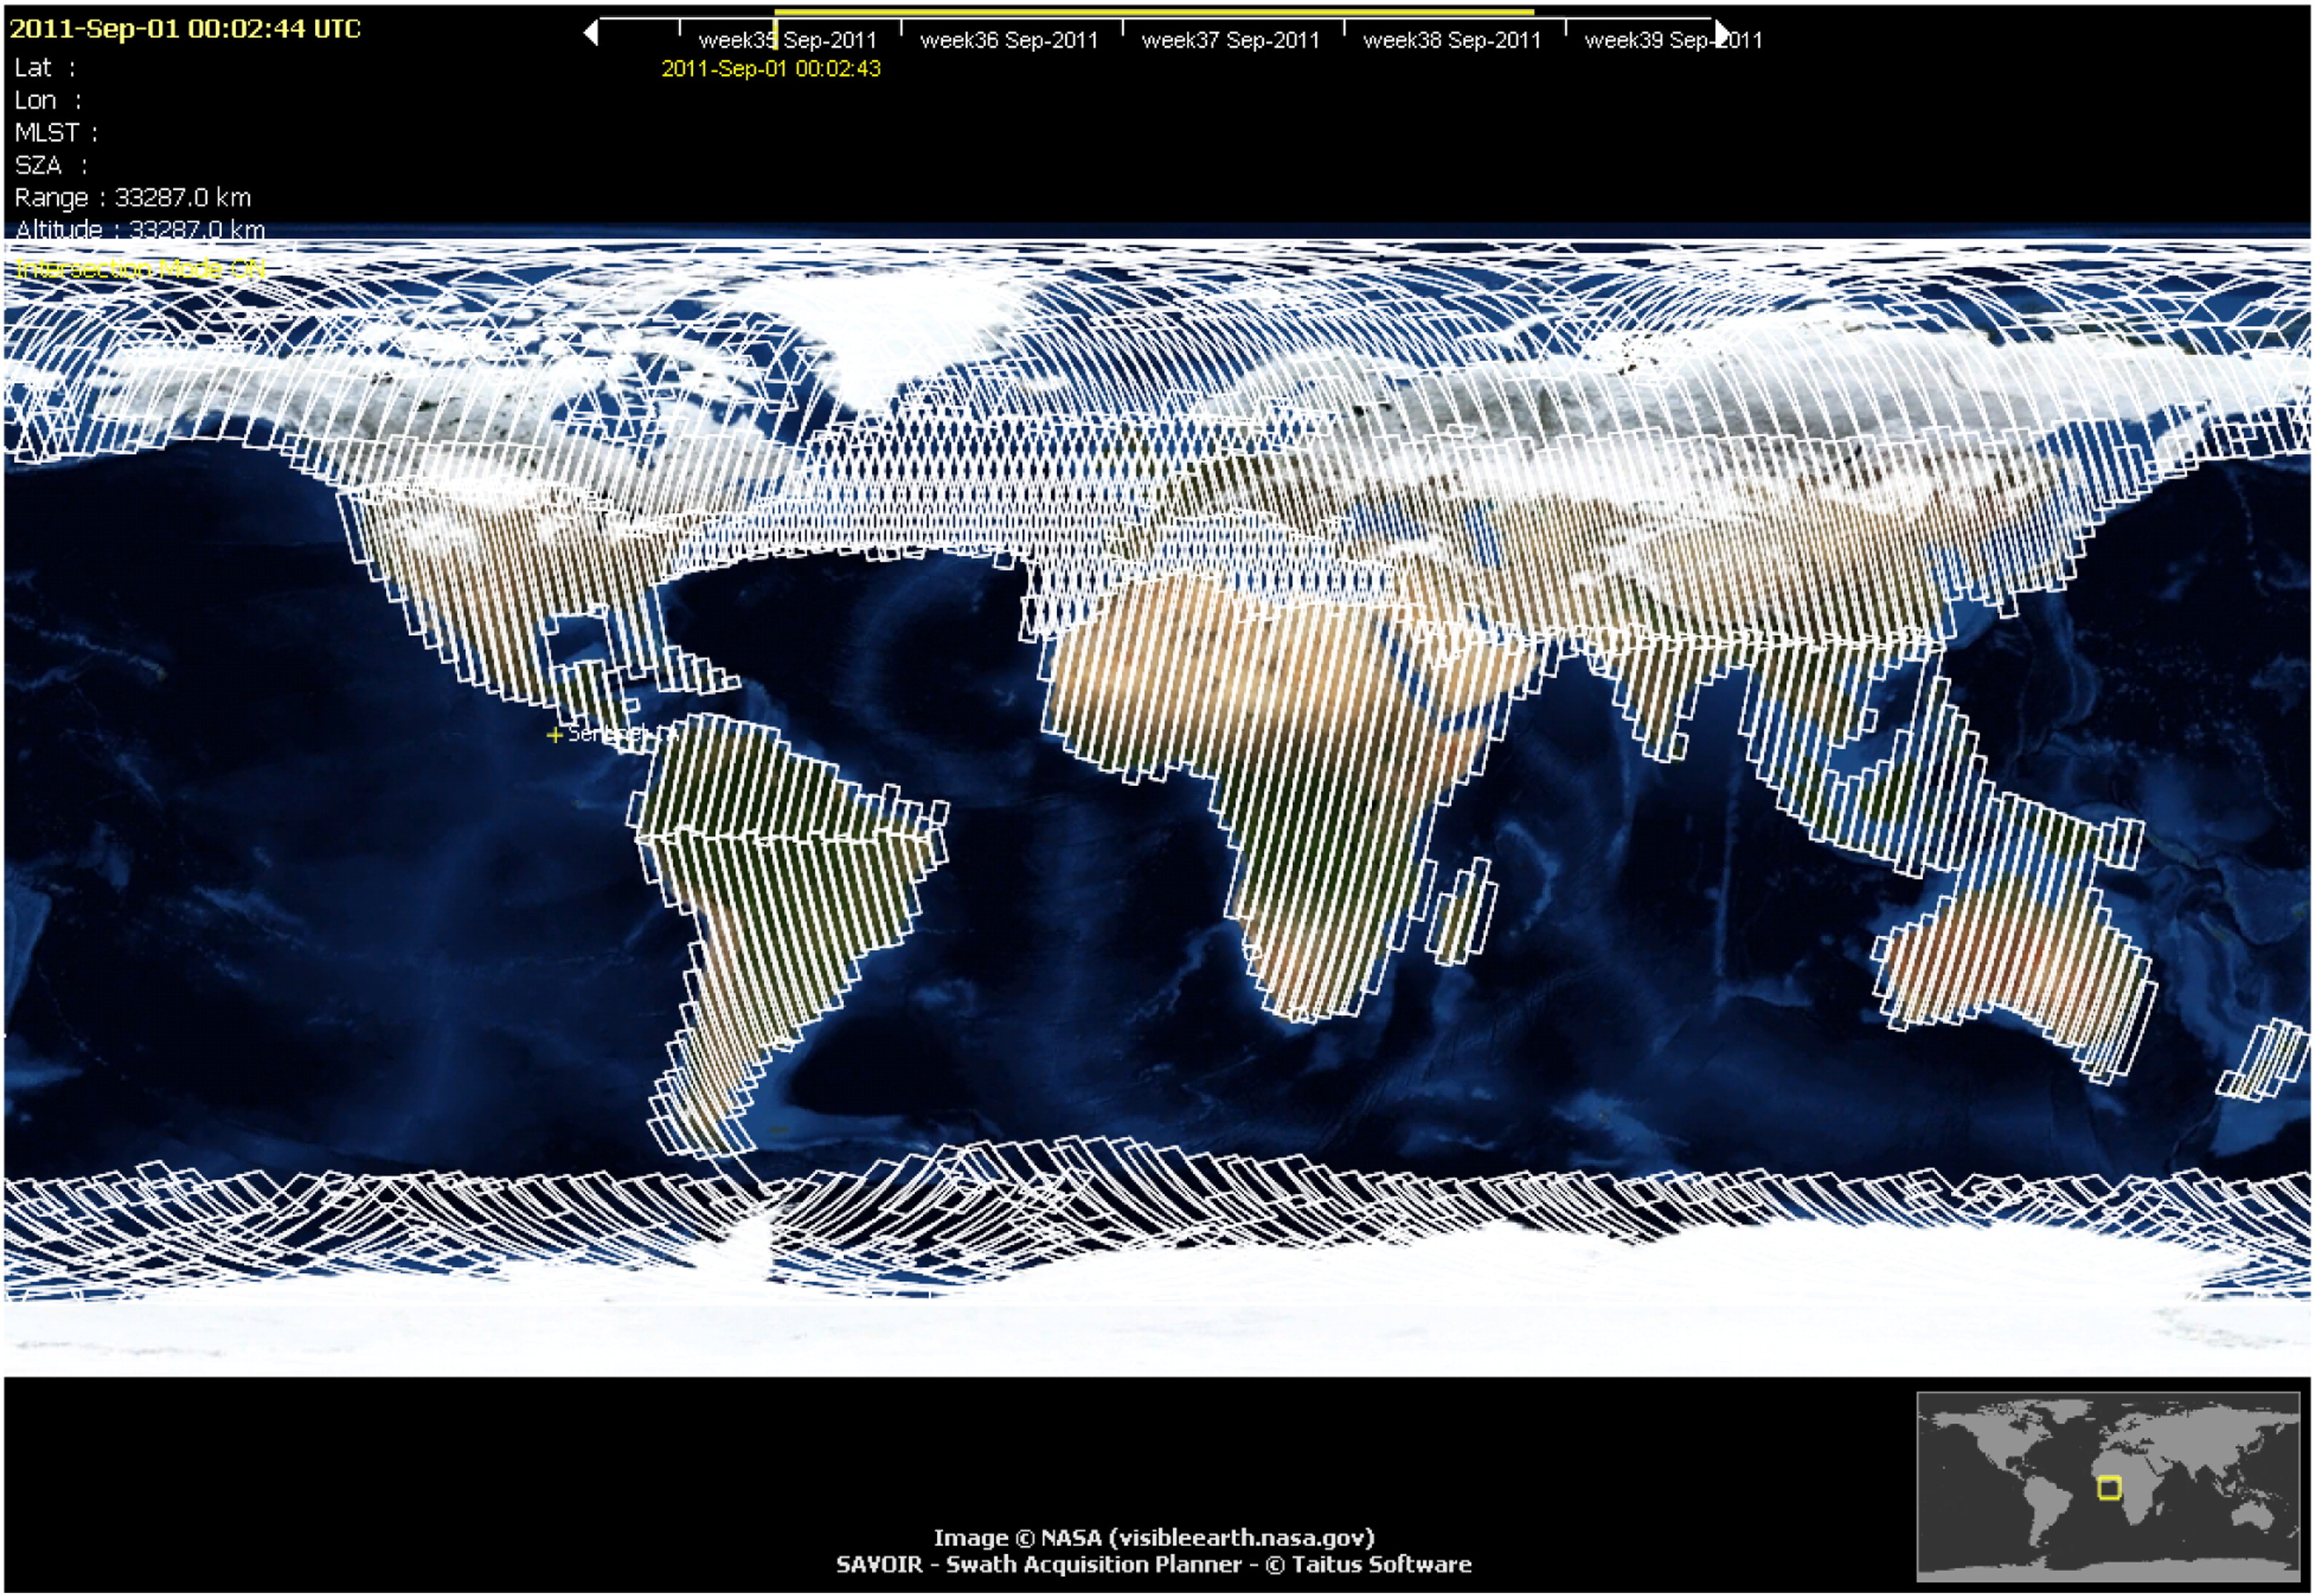
\includegraphics[width=.5\linewidth]{Figures/LiteratureReview/Satellites/sentinelCoverage.jpg}
    \caption{\ac{iw} mode coverage of one Sentinel-1 satellite after one 12-day orbit cycle. Taken from \cite{Torres2012b}.}
    \label{fig:litReview.sarCharac.satellites.sentinel.coverage}
\end{figure}

\begin{figure}[H]
	\centering
	\begin{subfigure}[t]{.48\linewidth}
		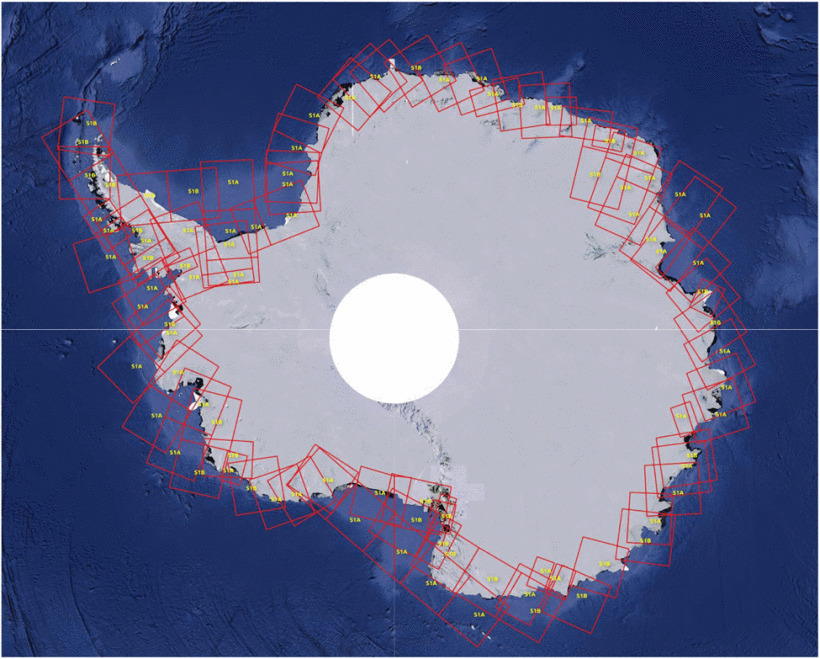
\includegraphics[width=\linewidth]{Figures/LiteratureReview/Satellites/sentinelCoverageCoast.jpg} 
 		\caption{Antarctic coastal coverage of Sentinel-1}
            \label{fig:litReview.sarCharac.satellites.sentinel.coverageCoast.sentinel}
	\end{subfigure}
	\hfill
	\begin{subfigure}[t]{.48\linewidth}
        \centering
		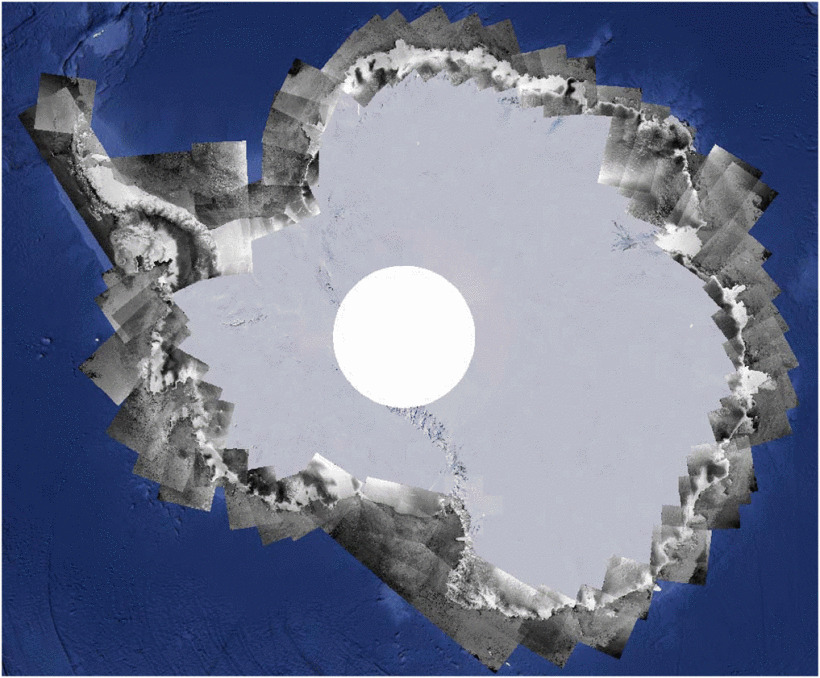
\includegraphics[width=0.98\linewidth]{Figures/LiteratureReview/Satellites/sentinelCoverageCoastMosaic.jpg} 
 		\caption{Constructed mosaic of the Antarctic coastline}
            \label{fig:litReview.sarCharac.satellites.sentinel.coverageCoast.mosaic}
	\end{subfigure}
    \caption{Antarctic coast line coverage and reconstructed continuous \acs{sar} image using Sentinel-1. Taken from \cite{Garkusha2020}.}
    \label{fig:litReview.sarCharac.satellites.sentinel.coverageCoast}
\end{figure}

Overall, the Sentinel-1 mission has been successful in capturing \acs{sar} data over Antarctica and the \acs{so}, as depicted in Figures \ref{fig:litReview.sarCharac.satellites.sentinel.coverage} and \ref{fig:litReview.sarCharac.satellites.sentinel.coverageCoast.sentinel}. Due to its open-source policy, the mission will be able to provide the desired data for this project.

\subsubsection{TerraSAR-X} \label{subsubsec:litReview.sarCharac.satellites.terraSAR}

The TerraSAR-X satellite is a German \acs{sar} satellite designed for scientific and commercial applications. It was launched on June 15, 2007 \cite{Werninghaus2004, Werninghaus2010}. TerraSAR-X continues the lineage of successful \acs{sar} missions initiated by \ac{nasa} and the \ac{asi}, notably X-SAR in 1994 and the \ac{srtm} in 2000, respectively \cite{Werninghaus2010}. The satellite is equipped with an active phased array antenna operating at X-Band frequency, capable of functioning in various modes\footnote{These modes include Spotlight, \acf{sm}, and Scan\acs{sar}. Additional modes, Staring Spotlight and Wide Scan\acs{sar}, were introduced after enhancements in 2013, which enhanced cross-range resolution and extended swath width respectively \cite{Buckreuss2018}.}. Moreover, TerraSAR-X supports multiple polarisations. The mission has two objectives: firstly, to provide the scientific community with multi-mode X-Band \acs{sar} data, and secondly, to foster the development of a commercial Earth Observation market in Europe \cite{Werninghaus2004}.

In terms of instrumentation, the satellite is equipped with 12 panels, each containing 32 dual-polarised waveguide subarrays. The centre frequency is 9.65\,GHz, and the system has a bandwidth of 300\,MHz. The antenna can operate in both H and V polarisations.\footnote{The meaning of these parameters is not crucial in this section of the report. Their significance and meaning will be further elaborated on in Chapter \ref{chap:theory}}.\cite{Werninghaus2004} Further details about satellite instrumentation can be found in references \cite{Werninghaus2004, Werninghaus2010}.

The orbit of TerraSAR-X is of interest for remote sensing of Antarctica. The mission is on a sun-synchronous orbit\footnote{See footnote 17} and orbits the Earth 15 2/11 times per day and has a repeat orbit every 11 days, or every 167 orbits \cite{Pitz2010}. The inclination of the orbit is important to ensure that the polar regions are captured, and as seen in Table \ref{tab:litReview.sarCharac.satellites.commonlyUsed}, the inclination of TerraSAR-X is 97.4\,$^{\circ}$. 

Buckreuss et al. \cite{Buckreuss2018} conducted a 10-year review of TerraSAR-X in 2018 and, when focusing on the total number of data acquisition requests over this period, found that over 30,000 left-looking data acquisitions out of the 226,000 acquisitions had been made. Buckreuss et al. stated that this benefits the scientific community, as it meant \acf{sm} acquisitions could be made over Antarctica. An image of these \acs{sm} acquisitions over Antarctica is shown in Figure \ref{fig:litReview.sarCharac.satellites.terraSAR.antarcticStripmaps}.

\begin{figure}[H]
    \centering
    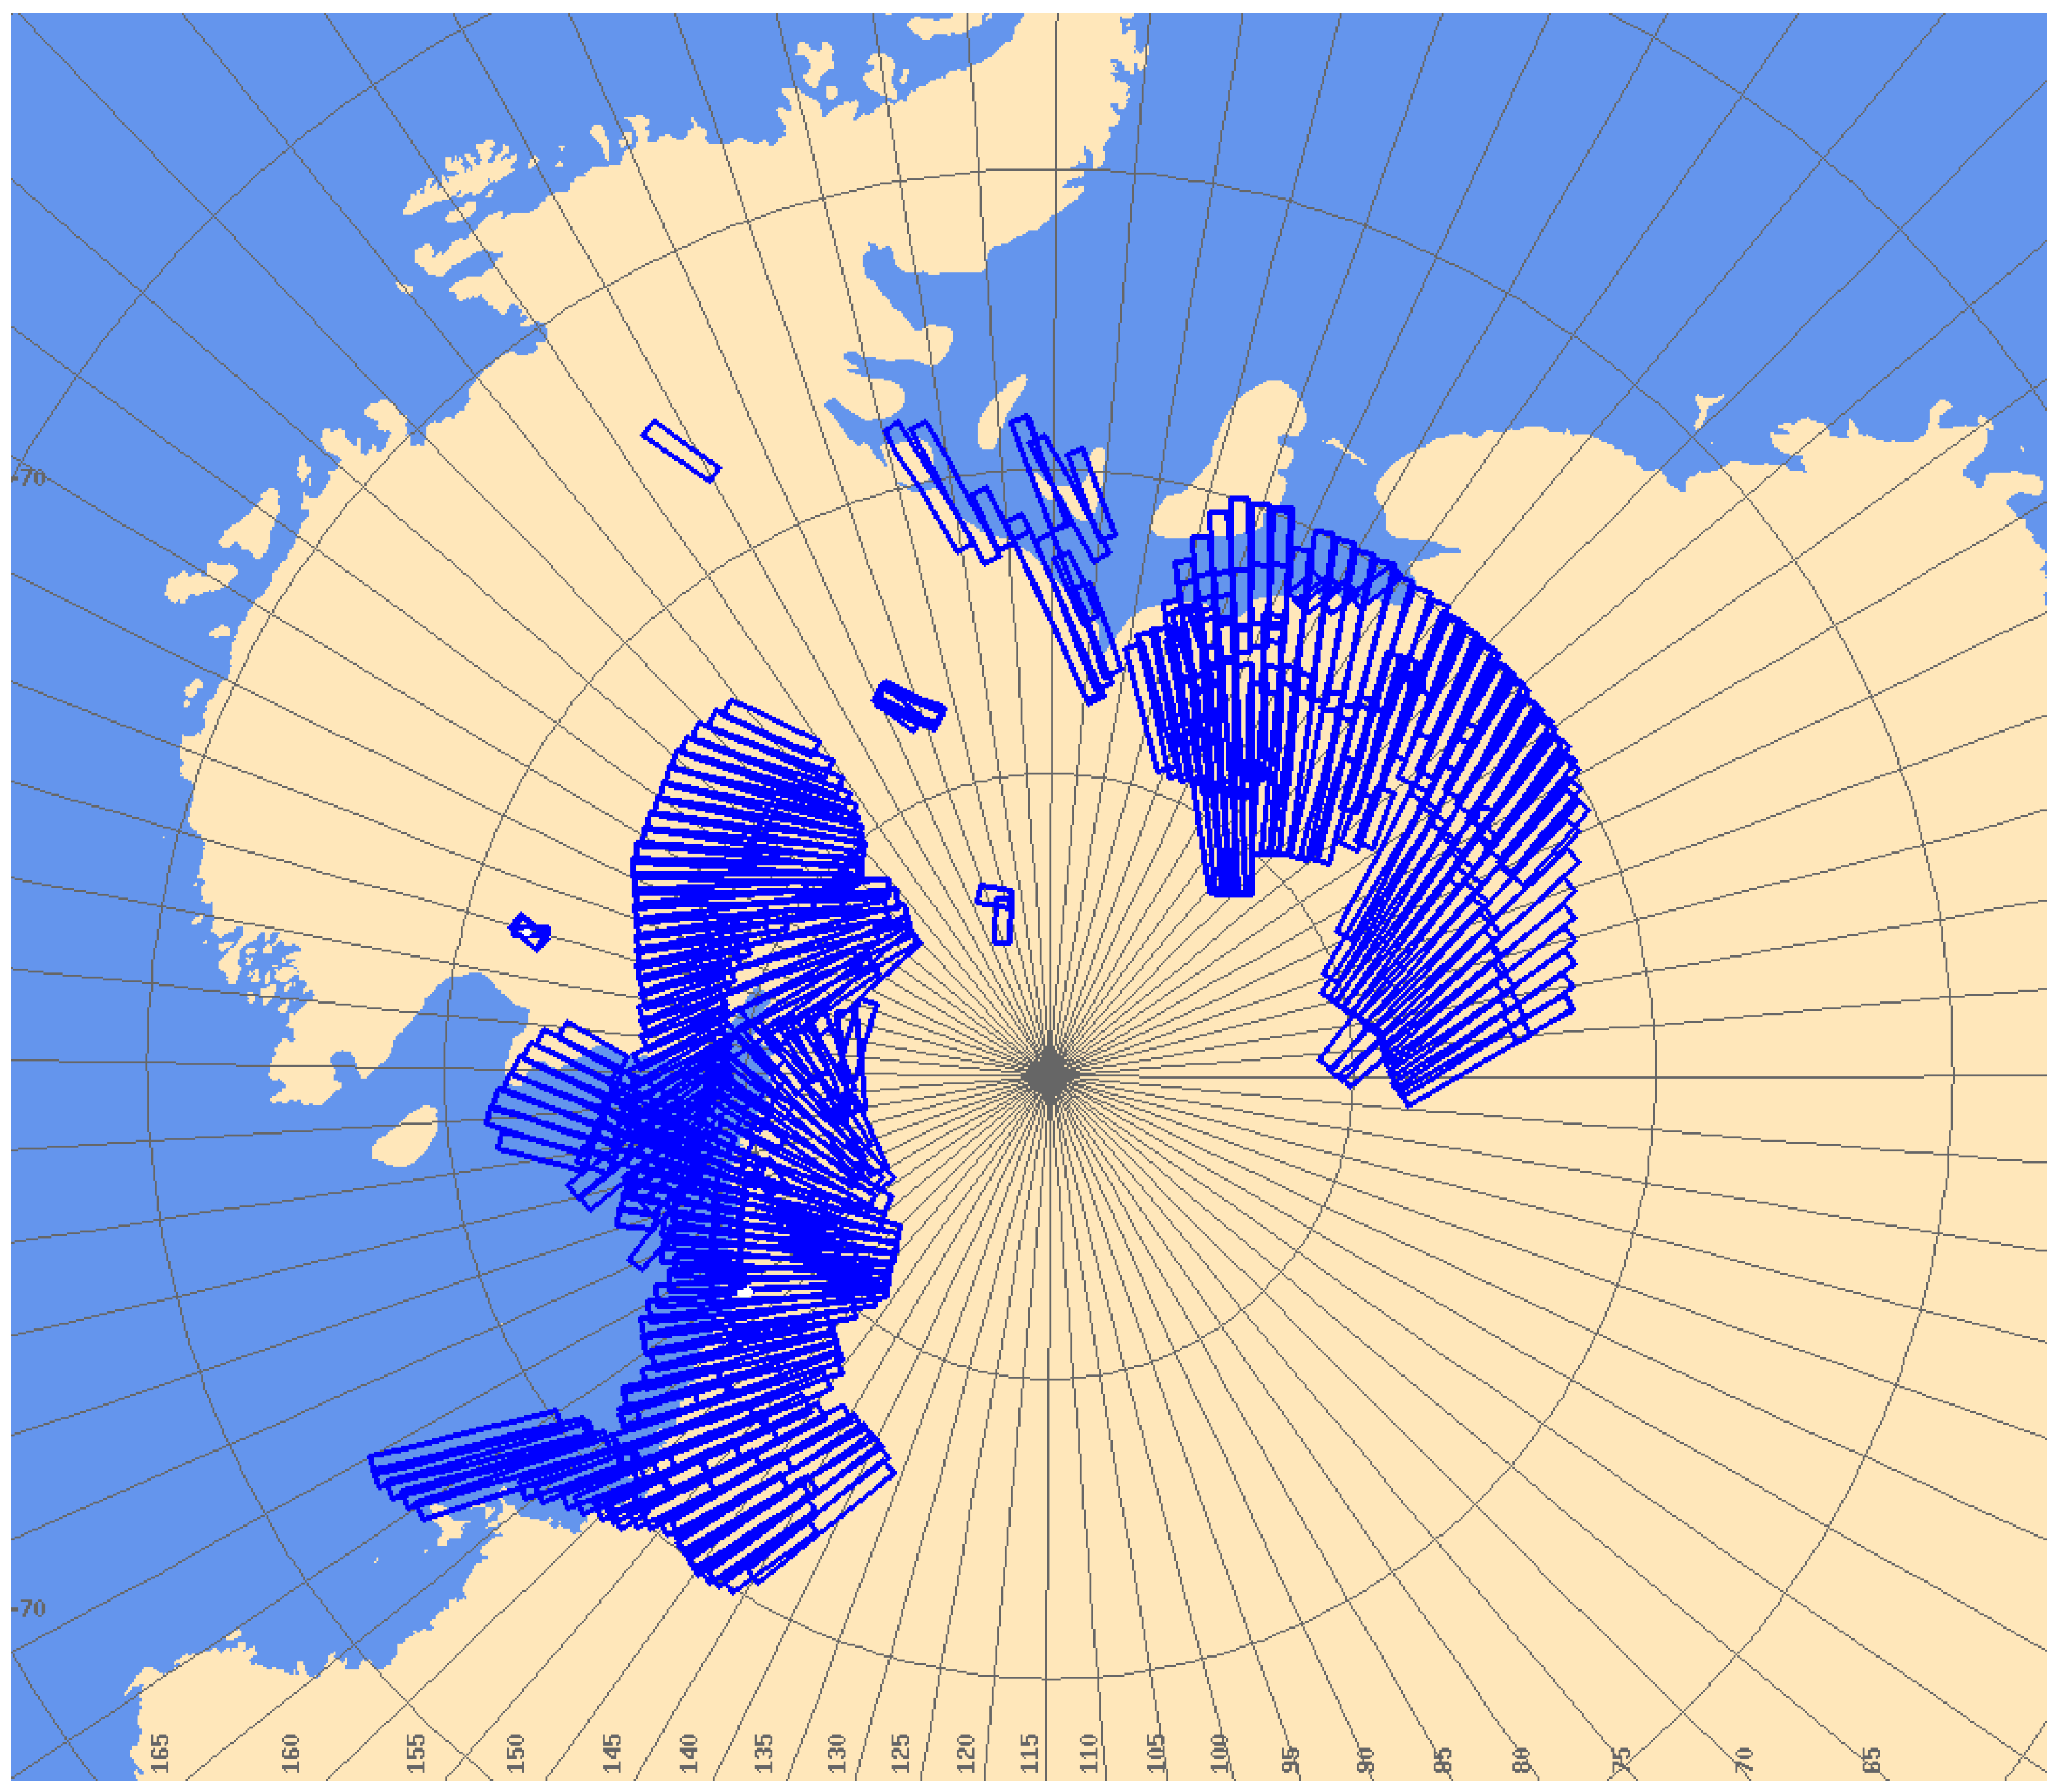
\includegraphics[width=.5\linewidth]{Figures/LiteratureReview/Satellites/TerraSAR_Antarctic_Acquisitions.png}
    \caption{Visualisation of the left-looking \ac{sm} acquisitions over Antarctica requested from TerraSAR-X. Taken from \cite{Buckreuss2018}}
    \label{fig:litReview.sarCharac.satellites.terraSAR.antarcticStripmaps}
\end{figure}

Buckreuss et al. \cite{Buckreuss2018} and Pitz and Miller \cite{Pitz2010} mention the launch of a second satellite, TanDEM-X, in 2010. This satellite can be used to perform bistatic operations in tandem with TerraSAR-X \cite{Pitz2010, Buckreuss2018}. However, these analysis techniques and methods fall outside the scope of this project.

Overall, the TerraSAR-X mission has been successful in capturing \acs{sar} data over Antarctica and the \acs{so}, as depicted in Figure \ref{fig:litReview.sarCharac.satellites.terraSAR.antarcticStripmaps}, and it will be able to provide the desired data for this project.

\subsection{SAR Ocean Wave Inversion} \label{subsec:litReview.sarCharac.oceanWaveInversion}

In order to convert a \acs{sar} spectrum into an directional wave spectrum, two main conversion methods are employed. The first technique is the Hasselmann inversion technique, originally proposed by \ac{hh} \cite{Hasselmann1991} in 1991, and further improved upon in 1996 by Hasselmann et al. \cite{Hasselmann1996}. The second technique, which builds upon the Hasselmann inversion, was developed by Engen and Johnsen \cite{Engen1995} in 1995. The theory encompassing these inversion techniques, along with the related wave spectra theory, is discussed in Chapter \ref{chap:theory}. This section will introduce the foundational aspects of these techniques, as well as their limitations. Subsequently, the following section will introduce the applications of these models in sea ice and wave modelling.

\subsubsection{Hasselmann Inversion Technique} \label{subsubsec:litReview.sarCharac.oceanWaveInversion.Hasselmann}

\ac{hh} developed a closed, nonlinear integral mapping transformation \cite{Wadhams2002}, which relates a \acs{sar} spectrum to a two-dimensional ocean-directional wave spectrum denoted as $E(\mathbf{k})$\footnote{$E(\mathbf{k})$ describes the distribution of wave energy with respect to the wave propagation number, $\mathbf{k}$. Further information about the two-dimensional wave spectrum is provided in Section \ref{subsec:theory.waves.waveSpectrum} and can be found in \cite{Hasselmann1991, Holthuijsen2007}.}. This wave spectrum enables the derivation of all statistical properties of an ocean wave field at any location and time \cite{Hasselmann1991}.

\ac{hh}'s inversion technique builds upon prior ocean inversion methods; however, these techniques were computationally inefficient and required a brute-force approach through the utilisation of Monte Carlo simulations\footnote{Monte Carlo simulations predict outcomes by employing estimated variable ranges and probability distributions. They iteratively generate results with various random numbers to produce a spectrum of likely scenarios.} for the statistical modelling of ocean waves using a pixel-by-pixel approach \cite{Hasselmann1991}.

\ac{hh} state that not all of the wave spectral information is mapped into the \acs{sar} image plane, and as such, they can only determine wave propagation direction to a specific sign \cite{Hasselmann1991}. Engen and Johsen \cite{Engen1995} overcome this limitation in the ways discussed in the following sub-section. This loss of information is due to two main issues. Firstly, the 180\,$^{\circ}$ propagation ambiguity\footnote{This ambiguity is due to the polarisation of the \acs{sar} waveform, as it does not allow the direction of the waves to be properly determined, i.e., whether they are travelling towards or away from a coastline or sea ice \cite{Fernandes2000}.}, and secondly, due to the nonlinear orbital motion of waves - particularly short waves and waves in windy oceans. This nonlinearity is known as velocity bunching and occurs due to fluctuations in the cross-range displacements of image backscattering elements, caused by changing orbital velocities within the wave field \cite{Hasselmann1991}. The nonlinearity in this relationship stems from the interference between wave orbital velocities and the way in which \acs{sar} constructs its cross-range resolution \cite{Mastenbroek2000}. \ac{hh} state that velocity bunching dominates over other nonlinearities and is the cause of smearing in the output \acs{sar} image spectrum \cite{Hasselmann1991}. This results in a loss of information for high wave numbers of the wave spectrum in the cross-range direction \cite{Hasselmann1991, Hasselmann1996}.

In order to mitigate these nonlinearities, \ac{hh} adopts the approach of utilising a first-guess wave spectrum, derived from an existing model of the sea state. Using this initial guess spectrum, \ac{hh}'s technique aims to minimise a cost function for extracting the wave spectrum. \ac{hh} has discovered that iterative minimisation of this cost function leads to convergence within 3-4 iterations \cite{Hasselmann1991}. While this approach to mitigating nonlinearities proved successful, it requires prior knowledge of the sea state. Consequently, several researchers have attempted to address this limitation using various methods. For instance, Engen and Johnsen's \cite{Engen1995} image cross-spectra technique, which is discussed in the subsequent sub-section.

\subsubsection{Image Cross Spectra Inversion Technique} \label{subsubsec:litReview.sarCharac.oceanWaveInversion.Engen}

Building on the \ac{hh} inversion technique, Engen and Johnsen were able to mitigate the 180\,$^{\circ}$ propagation ambiguity without using an existing first-guess wave model \cite{Engen1995}. This was achieved using image cross spectra [I still don't understand this technique entirely so want to understand it more before writing about it. I want to follow a similar form to the above sub-section though: What the technique is, how it differs and improves on Hasselmann's, a basic overview of the difference in approach it takes, and any limitations to the method]

\subsection{Wave Propagation Model in Sea Ice} \label{subsec:litReview.sarCharac.seaIceWaveModelling}

The process of modelling sea ice and waves is achieved through the use of three wave attenuation and dispersion models \cite{DeCarolis2021, DeSanti2018}. These models are crucial to Antarctic science, as they enable the assessment of wave attenuation rate, spreading, and dispersion within sea ice, which are closely linked to the physical characteristics of the sea ice itself. This, in turn, allows for the inference of sea ice's physical characteristics \cite{DeCarolis2002}.

These three models are the Keller model, developed in 1998 by Keller \cite{Keller1998}; the two-layer viscous model, developed in 2002 by De Carolis and Desiderio \cite{DeCarolis2002}; and the close-packing model, developed in 2017 by De Santi and Olla \cite{DeSanti2017}. More information on these models can be found in the respective references. These models can then be used to infer properties of the sea ice region, such as pancake ice thickness and wave attenuation rate \cite{Aulicino2019}. This sub-section will introduce each of these models, discuss their results when applied following the definition of an open ocean wave spectrum using either of the inversion techniques described in the above sub-section and state the difficulties and inaccuracies found within these models.

\subsubsection{Keller Model} \label{subsubsec:litReview.sarCharac.seaIceWaveModelling.Keller}

The Keller model \cite{Keller1998} views the ice layer as a suspension with a higher viscosity than the water it sits on top of, as well as a density slightly less than that of the water. The sea ice is treated as a highly viscous incompressible liquid, whereas the water underneath it is treated as an inviscid\footnote{An inviscid liquid has negligible or zero viscosity.} incompressible liquid. This allows breaking the problem down into a two-layer problem, for which linear theory can be applied to solve the dispersion equation for waves entering a sea ice field \cite{Keller1998}. Keller's model relies heavily on the effective viscosity coefficient, $\mu(c)$, which differs for different ice types based on their shape and concentration. The model has only two free parameters: the viscosity and thickness of the sea ice. The best values for these are found by minimising the difference between the observed and simulated \acs{sar} spectrum \cite{Wadhams2004}.

Keller's model improves on the previously used mass loading model since, at high wave frequencies, it fits laboratory experiments by predicting an increase in wave wavelength upon entering the sea ice. Furthermore, Wadhams et al. \cite{Wadhams2004} also found that the inferred thickness using Keller's model showed excellent agreement between calculated ice thickness and the average ice thickness from in-situ measurements in the \acs{miz}.

\subsubsection{Two-layer Viscous Model} \label{subsubsec:litReview.sarCharac.seaIceWaveModelling.twoLayer}

The two-layer viscous model \cite{DeCarolis2002} builds upon Keller's model due to the limitations inherent in Keller's model, which is constrained by specific approximations. This extension incorporates wave attenuation rate and dispersion as functions of wave frequency. Additionally, it introduces an eddy viscosity for the water beneath the sea ice, contributing to improved accuracy. The emergence of this eddy viscosity stems from the consideration of turbulence at the interface between the sea ice and the ocean, particularly at the base of the ice layer in order to parameterise water flow underneath sea ice \cite{DeCarolis2002,DeSanti2018}.

%De Carolis and Desiderio \cite{DeCarolis2002} represent pancake ice as a layer of viscous fluid \cite{DeCarolis2002,Doble2015}. This viscosity of the ice layer governs various interactions that occur when waves cross a region covered by pancake ice. Such interactions include bending and collisions among individual pancakes \cite{Doble2015}. Analogous to Keller's model, the two-layer viscous model maintains the premise that the ice layer exhibits higher viscosity than the underlying ocean, and it acknowledges the influence of ice density, dependent on ice type and concentration \cite{DeCarolis2002,Doble2015}. The two-layer viscous model has good agreement with laboratory results with regard to observed wave attenuation and dispersion in grease ice \cite{DeCarolis2002}. However, De Carolis and Desiderio states that whilst the inclusion of an eddy viscosity holds scientific value, it needs to be modelled using more robust numerical methods.

De Carolis and Desiderio \cite{DeCarolis2002} represent pancake ice as a layer of viscous fluid \cite{DeCarolis2002,Doble2015}. This viscosity of the ice layer governs various interactions that occur when waves cross a region covered by pancake ice, including bending and collisions among individual pancakes \cite{Doble2015}. Analogous to Keller's model, the two-layer viscous model maintains the premise that the ice layer exhibits a higher viscosity than the underlying ocean, and it acknowledges the influence of ice density, which is dependent on ice type and concentration \cite{DeCarolis2002,Doble2015}. The two-layer viscous model demonstrates good agreement with laboratory results concerning observed wave attenuation and dispersion in grease ice \cite{DeCarolis2002}. However, De Carolis and Desiderio \cite{DeCarolis2002} state that while the inclusion of an eddy viscosity holds scientific value, it needs to be modelled using more robust numerical methods for further validation.

\subsubsection{Close-Packing Model} \label{subsubsec:litReview.sarCharac.seaIceWaveModelling.CP}

[Still reading about this model. I want to follow a similar form to the two above subsections though. My idea is: The model it builds on and how it differs from this model (Any reasons for these choices in changes and improvements), a brief overview of how the model works, and any negatives to this approach when studied in comparison to in-situ measurements]

%****************************************************
% END
%****************************************************